\subsection{Analog-to-Digital Converter}

For at teste, hvorvidt ADC'em kan sample tre inputs, foretages en test, hvorpå 3 kanaler opsættes. Dette fremgår af \autoref{fig:treinput}.

\begin{figure}[H]
\centering
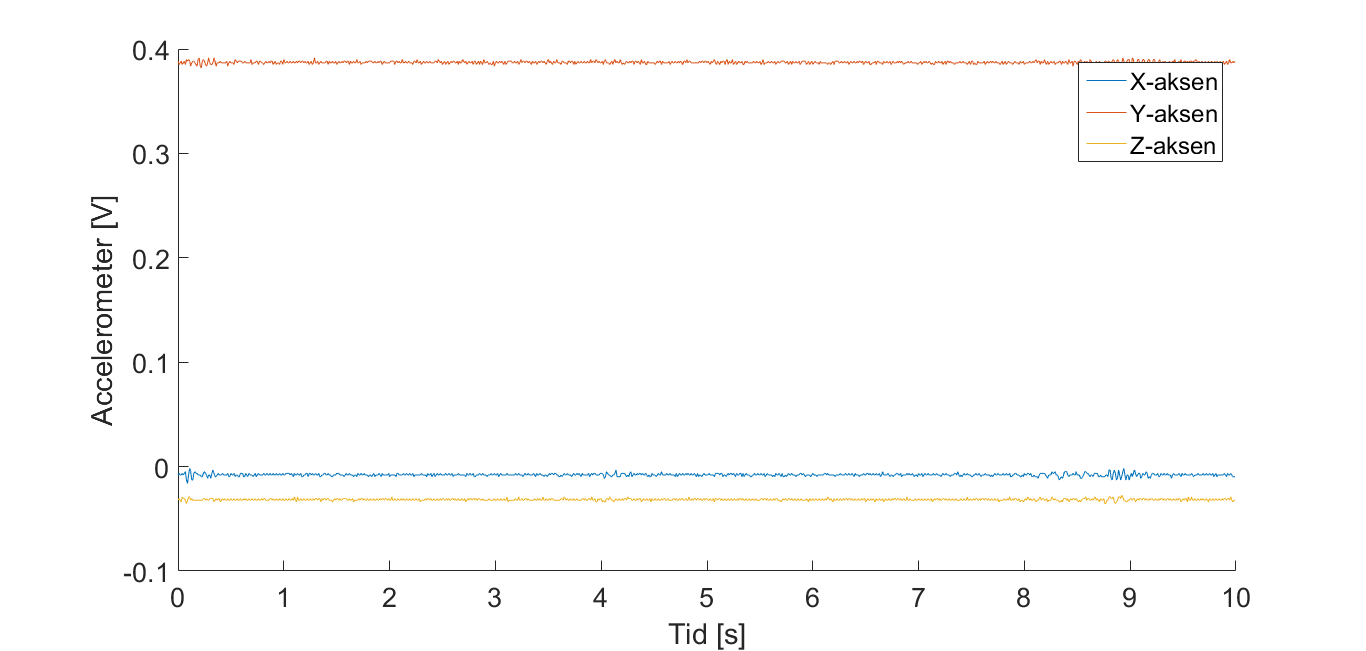
\includegraphics[width=1\textwidth]{figures/treinput}
\caption{Tre input samlpet samt visualiseret i MATLAB. Input-signalet er samplet fra acceleromterets tre akser.}
\label{fig:treinput}
\end{figure}

\noindent
Det ses af \autoref{fig:treinput}, at ADC'en herved kan sample 3 inputs fra et accelerometer. Kanalerne kan herved ændres til et ønsket inputsignal eksempelvis et muskelsignal. 

På baggrund af \autoref{sec:ADC_imp} er der valgt at anvende en ADC med et arbejdsområde på $2^{11}$, hvilket vurderes at være acceptabel og ikke forringer det ønskede signal under konverteringen. Dette ses ligeledes af \autoref{fig:treinput}.

Det fremgår \autoref{sec:pilotforsoeg} at frekvensområdet for muskelaktivitet befinder sig relativt lavfrekvent mellem $0,4-10~Hz$. Derved anses en samplingfrekvens på $100~Hz$ tilstrækkeligt. 

Derudover fremgår det af \autoref{fig:treinput}, at signalet ikke overstiger ADC'ens arbejdsområde under store udsving af accelerometersignalet. Hertil forventes det, at signalet ikke overstiger arbejdsområdet ved det endelige system, da bevægelsen herunder er kontrolleret og med mindre udsving.

ADC'ens samplingsfrekvens testes for at undersøge om den indstillede og reelle samplerate er identisk. Til denne test defineres en variable, som tæller op for hver gang, at der er konverteret data fra ADC'en. Hvis en konvertering mislykkes vil den givende sample ikke registreres. De registrerede værdier videresendes via USB-forbindelse mellem computer og mikrokontroller, hvorefter dataen aflæses i MATLAB. 
Testen foretages i 30 minutter, hvorved konverteringen samt tid startes på samme tid. De registrede data aflæses, hvorved en samplingsfrekvens udregnes af \autoref{eq:ADC_test}. Antallet af konverteringer målt under testen er $177066~samples$ over en periode af $1800,16~s$.

\begin{equation}\label{eq:ADC_test}
Fs = \frac{177066~samples}{1800,16~s}
\end{equation}

\noindent
Der forventes en samplingsfrekvens på $100~Hz$. Den reelle frekvens er udregnet til $98,36~Hz$ ud fra \autoref{eq:ADC_test}. Dette giver en afvigelse på $1,64\%$. Afvigelsen kan relateres til, at tiden og konverteringen ikke har været startet og stoppet på præcis samme tid. Dette resulterer i, at der ikke er en direkte relation mellem køretiden for ADC'en og tiden. Yderligere tillader indstillingerne for ADC'en, at der kan ændres i konverteringstiden for de enkelte kanaler, men samtidig oplyse, at der bevares en aktuel samplingsfrekvens på $100~Hz$. Dette antages ligeledes at have en indflydelse på samplingsfrekvensen, selvom den oplyses som værende $100~Hz$. 

Tiltrods for afvigelsen godkendes ADC'en indstillinger. Dette relateres til, at lavfrekvente signaler samples, og at størrelsen på afvigelsen ikke har betydning for repræsentationen af signalerne. 
Med henblik på den endelige anvendelse i form af et exoskellet, vil systemet ligeledes skulle følge kroppens naturlige bevægelse. Hertil fremhæves, at exoskelletet ikke skal tilpasse en ny position 100 gange i sekundet, da det ville være uhensigtsmæssigt.


\vspace{3mm}
\textbf{Opsummering af krav:}
\begin{itemize}
\item[\text{\sffamily \checkmark}] Skal sample minimum tre inputs 
\item[\text{\sffamily \checkmark}] Skal have en opløsning, der ikke forringer signalet
\item[\text{\sffamily \checkmark}] Skal undgå, at signalet ikke overstiger ADC'ens arbejdsområde
\item[\text{\sffamily \checkmark}] Skal have en samplingsfrekvens omkring 10 gange større end den højeste signalfrekvens
\item[\text{\sffamily \checkmark}] Samplingsfrekvensen skal have en maksimal afvigelse på $2~\%$
\end{itemize}

